% Options for packages loaded elsewhere
\PassOptionsToPackage{unicode}{hyperref}
\PassOptionsToPackage{hyphens}{url}
\documentclass[
  12pt,
  a4paper,
]{report}
\usepackage{xcolor}
\usepackage[margin=2cm]{geometry}
\usepackage{amsmath,amssymb}
\setcounter{secnumdepth}{5}
\usepackage{iftex}
\ifPDFTeX
  \usepackage[OT1]{fontenc}
  \usepackage[utf8]{inputenc}
  \usepackage{textcomp} % provide euro and other symbols
\else % if luatex or xetex
  \usepackage{unicode-math} % this also loads fontspec
  \defaultfontfeatures{Scale=MatchLowercase}
  \defaultfontfeatures[\rmfamily]{Ligatures=TeX,Scale=1}
\fi
\usepackage{lmodern}
\ifPDFTeX\else
  % xetex/luatex font selection
\fi
% Use upquote if available, for straight quotes in verbatim environments
\IfFileExists{upquote.sty}{\usepackage{upquote}}{}
\IfFileExists{microtype.sty}{% use microtype if available
  \usepackage[]{microtype}
  \UseMicrotypeSet[protrusion]{basicmath} % disable protrusion for tt fonts
}{}
\makeatletter
\@ifundefined{KOMAClassName}{% if non-KOMA class
  \IfFileExists{parskip.sty}{%
    \usepackage{parskip}
  }{% else
    \setlength{\parindent}{0pt}
    \setlength{\parskip}{6pt plus 2pt minus 1pt}}
}{% if KOMA class
  \KOMAoptions{parskip=half}}
\makeatother
\usepackage{color}
\usepackage{fancyvrb}
\newcommand{\VerbBar}{|}
\newcommand{\VERB}{\Verb[commandchars=\\\{\}]}
\DefineVerbatimEnvironment{Highlighting}{Verbatim}{commandchars=\\\{\}}
% Add ',fontsize=\small' for more characters per line
\newenvironment{Shaded}{}{}
\newcommand{\AlertTok}[1]{\textcolor[rgb]{1.00,0.00,0.00}{\textbf{#1}}}
\newcommand{\AnnotationTok}[1]{\textcolor[rgb]{0.38,0.63,0.69}{\textbf{\textit{#1}}}}
\newcommand{\AttributeTok}[1]{\textcolor[rgb]{0.49,0.56,0.16}{#1}}
\newcommand{\BaseNTok}[1]{\textcolor[rgb]{0.25,0.63,0.44}{#1}}
\newcommand{\BuiltInTok}[1]{\textcolor[rgb]{0.00,0.50,0.00}{#1}}
\newcommand{\CharTok}[1]{\textcolor[rgb]{0.25,0.44,0.63}{#1}}
\newcommand{\CommentTok}[1]{\textcolor[rgb]{0.38,0.63,0.69}{\textit{#1}}}
\newcommand{\CommentVarTok}[1]{\textcolor[rgb]{0.38,0.63,0.69}{\textbf{\textit{#1}}}}
\newcommand{\ConstantTok}[1]{\textcolor[rgb]{0.53,0.00,0.00}{#1}}
\newcommand{\ControlFlowTok}[1]{\textcolor[rgb]{0.00,0.44,0.13}{\textbf{#1}}}
\newcommand{\DataTypeTok}[1]{\textcolor[rgb]{0.56,0.13,0.00}{#1}}
\newcommand{\DecValTok}[1]{\textcolor[rgb]{0.25,0.63,0.44}{#1}}
\newcommand{\DocumentationTok}[1]{\textcolor[rgb]{0.73,0.13,0.13}{\textit{#1}}}
\newcommand{\ErrorTok}[1]{\textcolor[rgb]{1.00,0.00,0.00}{\textbf{#1}}}
\newcommand{\ExtensionTok}[1]{#1}
\newcommand{\FloatTok}[1]{\textcolor[rgb]{0.25,0.63,0.44}{#1}}
\newcommand{\FunctionTok}[1]{\textcolor[rgb]{0.02,0.16,0.49}{#1}}
\newcommand{\ImportTok}[1]{\textcolor[rgb]{0.00,0.50,0.00}{\textbf{#1}}}
\newcommand{\InformationTok}[1]{\textcolor[rgb]{0.38,0.63,0.69}{\textbf{\textit{#1}}}}
\newcommand{\KeywordTok}[1]{\textcolor[rgb]{0.00,0.44,0.13}{\textbf{#1}}}
\newcommand{\NormalTok}[1]{#1}
\newcommand{\OperatorTok}[1]{\textcolor[rgb]{0.40,0.40,0.40}{#1}}
\newcommand{\OtherTok}[1]{\textcolor[rgb]{0.00,0.44,0.13}{#1}}
\newcommand{\PreprocessorTok}[1]{\textcolor[rgb]{0.74,0.48,0.00}{#1}}
\newcommand{\RegionMarkerTok}[1]{#1}
\newcommand{\SpecialCharTok}[1]{\textcolor[rgb]{0.25,0.44,0.63}{#1}}
\newcommand{\SpecialStringTok}[1]{\textcolor[rgb]{0.73,0.40,0.53}{#1}}
\newcommand{\StringTok}[1]{\textcolor[rgb]{0.25,0.44,0.63}{#1}}
\newcommand{\VariableTok}[1]{\textcolor[rgb]{0.10,0.09,0.49}{#1}}
\newcommand{\VerbatimStringTok}[1]{\textcolor[rgb]{0.25,0.44,0.63}{#1}}
\newcommand{\WarningTok}[1]{\textcolor[rgb]{0.38,0.63,0.69}{\textbf{\textit{#1}}}}
\usepackage{longtable,booktabs,array}
\usepackage{caption}
\captionsetup[table]{skip=6pt}
\newcounter{none} % for unnumbered tables
\usepackage{calc} % for calculating minipage widths
% Correct order of tables after \paragraph or \subparagraph
\usepackage{etoolbox}
\makeatletter
\patchcmd\longtable{\par}{\if@noskipsec\mbox{}\fi\par}{}{}
\makeatother
\usepackage{graphicx}
\makeatletter
\newsavebox\pandoc@box
\newcommand*\pandocbounded[1]{% scales image to fit in text height/width
  \sbox\pandoc@box{#1}%
  \Gscale@div\@tempa{\textheight}{\dimexpr\ht\pandoc@box+\dp\pandoc@box\relax}%
  \Gscale@div\@tempb{\linewidth}{\wd\pandoc@box}%
  \ifdim\@tempb\p@<\@tempa\p@\let\@tempa\@tempb\fi% select the smaller of both
  \ifdim\@tempa\p@<\p@\scalebox{\@tempa}{\usebox\pandoc@box}%
  \else\usebox{\pandoc@box}%
  \fi%
}
% Set default figure placement to htbp
\def\fps@figure{htbp}
\makeatother
\setlength{\emergencystretch}{3em} % prevent overfull lines
\providecommand{\tightlist}{%
  \setlength{\itemsep}{0pt}\setlength{\parskip}{0pt}}
\DeclareUnicodeCharacter{00D7}{\ensuremath{\times}}
\DeclareUnicodeCharacter{2192}{\ensuremath{\rightarrow}}
\DeclareUnicodeCharacter{2265}{\ensuremath{\geq}}
\DeclareUnicodeCharacter{2264}{\ensuremath{\leq}}
\DeclareUnicodeCharacter{03C1}{\ensuremath{\rho}}
\DeclareUnicodeCharacter{2248}{\ensuremath{\approx}}
\usepackage{setspace}\onehalfspacing
\usepackage{float}
\floatplacement{figure}{H}
\usepackage{bookmark}
\IfFileExists{xurl.sty}{\usepackage{xurl}}{} % add URL line breaks if available
\urlstyle{same}
% fallback for those not using the hyperref driver hyperxmp:
\makeatletter
\@ifundefined{xmpquote}{\newcommand{\xmpquote}[1]{#1}}{}
\makeatother
\hypersetup{
  pdftitle={Learning What to Ignore: Deriving Invariance for Self-Supervised Text Recognition},
  hidelinks,
  pdfcreator={LaTeX via pandoc}}

\title{Learning What to Ignore: Deriving Invariance for Self-Supervised
Text Recognition}
\author{}
\date{}

\begin{document}
\maketitle

{
\setcounter{tocdepth}{2}
\tableofcontents
}
\listoffigures
\listoftables
\chapter{Introduction}\label{introduction}

\section{Background}\label{background}

Handwritten text recognition (HTR) is the task of reading the characters
in an image of handwriting and producing the matching typed text. Most
practical systems work on one text line at a time: a page is first split
into lines, and a recogniser maps each line image to a character
sequence. A widely used design is the convolutional recurrent neural
network (CRNN) {[}1{]}, in which a convolutional network (CNN) extracts
visual features along the line, a bidirectional LSTM models the order of
characters, and connectionist temporal classification (CTC) aligns the
output with the target text without needing the position of each
character.

On clean modern handwriting such as the IAM database {[}2{]}, these
recognisers are accurate. Historical documents are a different setting.
Centuries-old manuscripts, such as those collected in CATMuS Medieval
{[}3{]}, show faded or corroded ink, darkened and uneven paper, ink from
the reverse side showing through, stains, and blur or noise from the
scanning process. Each of these changes the image without changing the
text, and each can raise the error of a recogniser that never saw it
during training.

The usual remedy is more labelled data, that is, more line images with
typed transcriptions. For damaged historical collections this is
expensive: a transcriber needs palaeographic training, and the most
damaged lines are the slowest to transcribe. Self-supervised learning
(SSL) offers a way around this. A model first learns from unlabelled
lines through a pretext task, such as rebuilding hidden parts of an
image, and is then fine-tuned on the few labelled lines that exist
{[}4{]}, {[}5{]}, {[}6{]}. For handwriting, recent work shows that
pixel-reconstruction methods such as masked autoencoders {[}7{]}
outperform contrastive methods {[}8{]}.

Every SSL method, however, depends on a choice that is rarely examined:
which variations the model should learn to ignore. This is set through
the augmentations or corruptions applied during pretraining, and for
text it is usually a hand-picked list whose strengths are tuned by trial
and error. This project asks whether that list can instead be derived
from measurements of real damaged documents, and whether doing so helps
a recogniser read them.

\section{Applications and Target
Users}\label{applications-and-target-users}

The work is aimed at people who need machine-readable text from damaged
handwritten collections but cannot afford to transcribe thousands of
lines by hand:

\begin{itemize}
\tightlist
\item
  \textbf{Archives, libraries and museums} that digitise manuscript
  collections and want searchable full text, not only page images.
\item
  \textbf{Digital-humanities researchers} who build editions and corpora
  from historical sources and use HTR platforms such as Transkribus or
  eScriptorium, where a new collection usually starts with very few
  transcribed lines.
\item
  \textbf{Developers of HTR tools}, who must decide which augmentations
  to ship for a new collection. A measured damage recipe replaces
  guesswork with a repeatable procedure.
\end{itemize}

The pilot results in Chapter 6 give concrete numbers for this setting. A
commercial off-the-shelf recogniser (PaddleOCR PP-OCRv6 {[}9{]}) reads
clean IAM lines with an 11.4\% character error rate (CER) but medieval
CATMuS lines with 52.5\% CER. A small CRNN trained on all 23,762 CATMuS
training lines reaches 20.0\% CER, but with only 5\% of those labels
(1,188 lines) the error rises to 33.8\%. On IAM, reducing the labels
from 10\% to 1\% raises the error from 19.9\% to 43.3\%. Few labels and
damaged pages together are therefore the case where current tools fail,
and it is the case this project targets.

\section{Scope}\label{scope}

Phase 1 focuses on a single question: which damage should a line
recogniser learn to see through? It works on single text lines, small
models that train on one 8 GB laptop GPU, seven damage types, and two
datasets in the Latin script. Page layout analysis, large
vision-language models and multilingual training are out of scope.
Transfer to an unseen script is planned as a later stretch test; until
then, all claims are limited to the Latin script.

\chapter{Problem Statement}\label{problem-statement}

\section{Statement}\label{statement}

Text recognisers fail on damaged documents, and damaged documents are
exactly where labelled training data is scarcest. Self-supervised
learning can use unlabelled lines, but it must be told which variations
to ignore, and today that choice is a hand-picked list of corruptions
re-tuned for every new collection. This project derives the choice from
the documents themselves: it measures the main damage types on real
historical lines, sets the frequency and strength of synthetic damage
from those measurements, trains with it, and tests whether the learned
invariance transfers to unseen damage, media and scripts, and whether it
predicts where recognition fails.

\section{Research Questions and
Hypotheses}\label{research-questions-and-hypotheses}

Each question is stated with the result that would show our claim to be
wrong. These rules were fixed before any experiments were run.

\begin{longtable}[]{@{}
  >{\raggedright\arraybackslash}p{(\linewidth - 4\tabcolsep) * \real{0.3333}}
  >{\raggedright\arraybackslash}p{(\linewidth - 4\tabcolsep) * \real{0.3333}}
  >{\raggedright\arraybackslash}p{(\linewidth - 4\tabcolsep) * \real{0.3333}}@{}}
\caption{Research questions, hypotheses and the result that would refute
each.}\tabularnewline
\toprule\noalign{}
\begin{minipage}[b]{\linewidth}\raggedright
\end{minipage} & \begin{minipage}[b]{\linewidth}\raggedright
Question and claim
\end{minipage} & \begin{minipage}[b]{\linewidth}\raggedright
The claim is wrong if
\end{minipage} \\
\midrule\noalign{}
\endfirsthead
\toprule\noalign{}
\begin{minipage}[b]{\linewidth}\raggedright
\end{minipage} & \begin{minipage}[b]{\linewidth}\raggedright
Question and claim
\end{minipage} & \begin{minipage}[b]{\linewidth}\raggedright
The claim is wrong if
\end{minipage} \\
\midrule\noalign{}
\endhead
\bottomrule\noalign{}
\endlastfoot
RQ1 (H1) & Does damage derived from real pages beat plain masking and
hand-picked damage when few labels exist? Claim: it lowers the error on
real historical lines. & the gap is within the spread across random
seeds, or hand-picked damage matches it \\
RQ2 (H2) & What transfers? Claim: the benefit shrinks with distance from
what was fitted: first an unseen damage type, then a new medium, then a
new script. & transfer to a new script equals or beats transfer to a new
damage type \\
RQ3 (H3) & Does a model's invariance to a damage type predict how much
that damage raises its error? Claim: ignoring damage that touches only
the paper helps, while ignoring damage on the strokes does not (a ``sign
flip''). & a single relationship holds for all damage types, or there is
none \\
\end{longtable}

\chapter{Literature Survey}\label{literature-survey}

\section{Self-Supervised Learning for Text
Recognition}\label{self-supervised-learning-for-text-recognition}

Penarrubia, Valero-Mas and Calvo-Zaragoza {[}4{]} review SSL for both
handwritten and scene text. They group methods into discriminative ones
(contrastive learning, distillation, clustering and others) and
generative ones (masked image modelling, inpainting), and they report
that results are hard to compare because papers use different evaluation
protocols and label fractions. They also stress that augmentations must
suit text: a horizontal flip or a random crop can destroy the reading
order. The survey maps the field but gives no procedure for choosing
augmentations.

SeqCLR {[}10{]} adapted contrastive learning to text by treating a line
as a sequence of frames and contrasting matching frames across two
augmented views. LoGo-HTR {[}11{]} combines a local contrastive loss
with a global decorrelation loss, pretrains on about ten million word
images, and reports gains over earlier methods with only a fraction of
the labels. Neither studies document damage.

Lacuna Reconstruction {[}6{]} pretrains on unlabelled historical lines
by masking regions and asking the model to identify the hidden content
among distractors. With only 30 labelled lines, it reduces CER from
60.4\% to 23.7\%, using about 750,000 unlabelled lines. Kišš and Hradiš
{[}5{]} pretrain recognisers on unlabelled historical lines with
masked-prediction and joint-embedding objectives, then fine-tune with
varying amounts of labels. Pretraining clearly beats training from
scratch, but it struggles to beat supervised transfer from a related
labelled dataset. This is an important warning: SSL is not a guaranteed
gain, so a supervised baseline must always be reported.

Garrido-Munoz and Calvo-Zaragoza {[}8{]} compare six SSL methods from
three families under one encoder and protocol on six handwriting
benchmarks. Pixel reconstruction gives the lowest error on every
benchmark, which they explain by showing that the information that
separates characters lies in the high-variance pixel directions that
reconstruction must model. This result is why our project uses
reconstruction pretraining and asks \emph{which damage} rather than
\emph{which SSL family}.

Text-DIAE {[}12{]} is the closest earlier work. It trains an autoencoder
to undo masking, blur and noise, giving features that are robust to
these degradations for both recognition and document enhancement. The
degradations and their strengths are, however, chosen by hand, and
transfer to held-out damage types is not tested.

\section{Modelling Document Damage}\label{modelling-document-damage}

Degradation modelling for documents has a long history. Kanungo,
Haralick, Baird and co-authors {[}13{]} proposed a statistical method
for validating degradation models against real scans: synthetic pages
are accepted when their statistics are indistinguishable from real ones.
Baird {[}14{]} later reviewed the state of the art of such models. These
works targeted classical OCR on binary printed pages and were not
connected to what a deep recogniser learns to ignore.

Modern tools generate realistic damage at scale. Augraphy {[}15{]} is a
library of ink, paper and lighting effects arranged as a pipeline that
follows the life of a document. PreP-OCR {[}16{]} trains an image
restoration model on synthetic damage, runs OCR on the restored image
and corrects the output with a language model, reporting a 63.9--70.3\%
reduction in character error compared with OCR on the raw pages. In
both, which damage to use and how strong it should be is left to the
user, and the goal is restoration rather than training a recogniser that
ignores the damage.

\section{Invariance and Robustness}\label{invariance-and-robustness}

Ericsson, Gouk and Hospedales {[}17{]} measure how invariant a
self-supervised model is to each augmentation and show that different
downstream tasks need different invariances. Their measure, the
similarity of features for an image and its augmented version, is the
basis of the invariance measure used in this project. Mintun, Kirillov
and Xie {[}18{]} show that, for supervised image classifiers, the
similarity between training augmentations and test corruptions predicts
robustness. Both studies use natural images; neither derives the
corruptions from data or studies text.

\chapter{Research Gap and Objectives}\label{research-gap-and-objectives}

\section{Research Gap}\label{research-gap}

Each part of this project exists separately in earlier work. Damage
models have been fitted to scans {[}13{]}, damage libraries exist
{[}15{]}, degradation-invariant pretraining has been tried {[}12{]}, and
invariance can be measured {[}17{]}. What is missing is the link between
them:

\begin{enumerate}
\def\labelenumi{\arabic{enumi}.}
\tightlist
\item
  \textbf{The corruptions are hand-picked.} SSL methods for text
  {[}10{]}, {[}6{]}, {[}11{]} choose what the model should ignore by
  hand and re-tune it for each collection. We derive it from
  measurements of real damage.
\item
  \textbf{Fitted damage was never linked to deep recognisers.} Classical
  validation {[}13{]}, {[}14{]} was built for binary OCR. We connect the
  chain \emph{measured damage → recipe → what the model ignores → error
  on real damaged lines}.
\item
  \textbf{No held-out tests.} Damage-style augmentation in text SSL
  {[}12{]} is not tested on damage types, media or scripts held out from
  training. We hold out whole damage types, media and scripts.
\item
  \textbf{Nobody checks whether the choice matters.} Damage generators
  {[}15{]}, {[}16{]} leave the choice of damage to the user. We test
  whether what the model ignores predicts the error for each damage
  type.
\end{enumerate}

\section{Challenges}\label{challenges}

\begin{longtable}[]{@{}
  >{\raggedright\arraybackslash}p{(\linewidth - 4\tabcolsep) * \real{0.3333}}
  >{\raggedright\arraybackslash}p{(\linewidth - 4\tabcolsep) * \real{0.3333}}
  >{\raggedright\arraybackslash}p{(\linewidth - 4\tabcolsep) * \real{0.3333}}@{}}
\caption{Main challenges and how they are handled.}\tabularnewline
\toprule\noalign{}
\begin{minipage}[b]{\linewidth}\raggedright
Challenge
\end{minipage} & \begin{minipage}[b]{\linewidth}\raggedright
Why it matters
\end{minipage} & \begin{minipage}[b]{\linewidth}\raggedright
How it is handled
\end{minipage} \\
\midrule\noalign{}
\endfirsthead
\toprule\noalign{}
\begin{minipage}[b]{\linewidth}\raggedright
Challenge
\end{minipage} & \begin{minipage}[b]{\linewidth}\raggedright
Why it matters
\end{minipage} & \begin{minipage}[b]{\linewidth}\raggedright
How it is handled
\end{minipage} \\
\midrule\noalign{}
\endhead
\bottomrule\noalign{}
\endlastfoot
SSL may not beat supervised training {[}5{]} & The main use of the
recipe would be lost & A supervised baseline is always run; the
invariance analysis is a result either way, and the recipe is also
tested as augmentation \\
``You only learned your own simulator'' & A model trained on synthetic
damage may not read real damage & Testing is always done on real damaged
lines, grouped by measured damage \\
Some damage has no exact physical model & Fading and stains cannot be
written as exact formulas & Physical models where possible
(show-through, capture); the rest are labelled approximate \\
\end{longtable}

\section{Objectives}\label{objectives}

\begin{enumerate}
\def\labelenumi{\arabic{enumi}.}
\tightlist
\item
  Build a reproducible line-recognition pipeline with strong supervised
  baselines on clean and historical data.
\item
  Build a per-line damage measurement tool and quantify how real
  historical lines differ from clean ones.
\item
  Implement damage models whose frequency and strength are derived from
  these measurements.
\item
  Compare masked-autoencoder pretraining with derived damage against no
  damage, plain masking, hand-picked damage and a VICReg {[}19{]}
  control, and test the derived damage as training augmentation.
\item
  Test transfer to a held-out damage type, a new medium and an unseen
  script.
\item
  Relate each model's invariance to each damage type to the rise in
  error caused by that damage.
\end{enumerate}

\chapter{Overview of Datasets}\label{overview-of-datasets}

\section{Description}\label{description}

\begin{longtable}[]{@{}
  >{\raggedright\arraybackslash}p{(\linewidth - 8\tabcolsep) * \real{0.2000}}
  >{\raggedright\arraybackslash}p{(\linewidth - 8\tabcolsep) * \real{0.2000}}
  >{\raggedright\arraybackslash}p{(\linewidth - 8\tabcolsep) * \real{0.2000}}
  >{\raggedright\arraybackslash}p{(\linewidth - 8\tabcolsep) * \real{0.2000}}
  >{\raggedright\arraybackslash}p{(\linewidth - 8\tabcolsep) * \real{0.2000}}@{}}
\caption{Datasets used and planned.}\tabularnewline
\toprule\noalign{}
\begin{minipage}[b]{\linewidth}\raggedright
Dataset
\end{minipage} & \begin{minipage}[b]{\linewidth}\raggedright
Script
\end{minipage} & \begin{minipage}[b]{\linewidth}\raggedright
Size
\end{minipage} & \begin{minipage}[b]{\linewidth}\raggedright
Role
\end{minipage} & \begin{minipage}[b]{\linewidth}\raggedright
Status
\end{minipage} \\
\midrule\noalign{}
\endfirsthead
\toprule\noalign{}
\begin{minipage}[b]{\linewidth}\raggedright
Dataset
\end{minipage} & \begin{minipage}[b]{\linewidth}\raggedright
Script
\end{minipage} & \begin{minipage}[b]{\linewidth}\raggedright
Size
\end{minipage} & \begin{minipage}[b]{\linewidth}\raggedright
Role
\end{minipage} & \begin{minipage}[b]{\linewidth}\raggedright
Status
\end{minipage} \\
\midrule\noalign{}
\endhead
\bottomrule\noalign{}
\endlastfoot
IAM-line {[}2{]} & Latin (modern English) & 6,482 train / 976 val /
2,915 test lines; 657 writers & Clean baseline; base for synthetic
damage & Processed \\
CATMuS Medieval {[}3{]} & Latin (medieval Latin, French and others) &
About 195,000 lines in the current release & Real damage: measurement,
pretraining, testing & Subset processed \\
IIIT-INDIC-HW-WORDS {[}20{]} & 8 Indian scripts & 872,000 word images &
Optional script-transfer test & Planned \\
Muharaf {[}21{]} & Arabic & 36,311 manuscript lines (1,216 of 1,644
pages public) & Unseen-script stretch test & Planned \\
\end{longtable}

\textbf{IAM} contains modern English handwriting from 657 writers, with
text taken from the LOB corpus. We use the line-level release on Hugging
Face (Teklia), whose split is writer-independent: no writer appears in
both training and test. IAM is licensed for non-commercial research use.

\textbf{CATMuS Medieval} collects manuscripts and early printed books
from the 8th to the 16th century in about ten languages, transcribed
under shared guidelines. It is released under CC BY 4.0. Because the
full release is about 22.5 GB, the pilot uses a subset: Latin and French
lines from 11 projects, giving 23,762 training, 1,243 validation and
4,022 test lines. The test lines come from manuscripts that do not
appear in training, so the test measures generalisation to unseen
manuscripts. Shards were drawn round-robin across projects to keep the
subset varied.

\begin{figure}
\centering
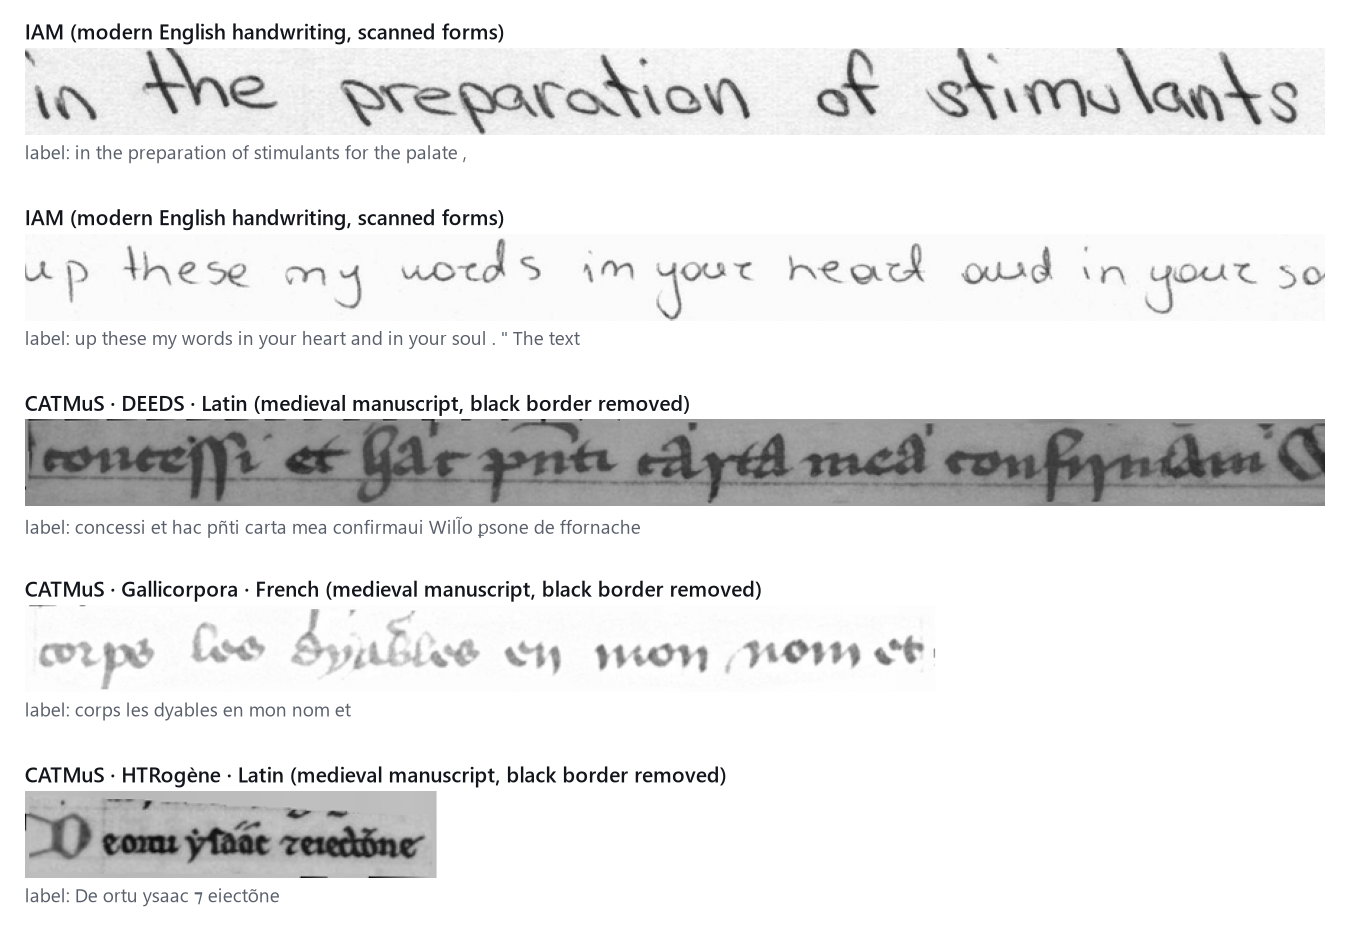
\includegraphics[width=0.8\linewidth,height=\textheight,keepaspectratio,alt={Sample
lines: modern handwriting from IAM (top two) and medieval manuscript
lines from three CATMuS projects (bottom three), with their
transcriptions.}]{figures/samples_iam_catmus.png}
\caption{Sample lines: modern handwriting from IAM (top two) and
medieval manuscript lines from three CATMuS projects (bottom three),
with their transcriptions.}
\end{figure}

\section{Data Attributes and
Features}\label{data-attributes-and-features}

\textbf{Pre-processing.} Every line is converted to grey-scale, resized
to a height of 64 pixels with its aspect ratio kept, and paired with its
transcription in Unicode NFC form. Character sets are built from the
training splits only: 79 symbols for IAM and 195 for CATMuS.

\textbf{Damage statistics.} For each line we compute eight statistics.
Six track a damage type; two (stroke width and ink fraction) mainly
reflect pen size and are treated as scale, not damage. Table 5.2
compares 3,000 sampled CATMuS lines with IAM using the
Kolmogorov--Smirnov distance D (0 means identical distributions, 1 means
completely separate).

\begin{longtable}[]{@{}
  >{\raggedright\arraybackslash}p{(\linewidth - 8\tabcolsep) * \real{0.2000}}
  >{\raggedright\arraybackslash}p{(\linewidth - 8\tabcolsep) * \real{0.2000}}
  >{\raggedright\arraybackslash}p{(\linewidth - 8\tabcolsep) * \real{0.2000}}
  >{\raggedright\arraybackslash}p{(\linewidth - 8\tabcolsep) * \real{0.2000}}
  >{\raggedright\arraybackslash}p{(\linewidth - 8\tabcolsep) * \real{0.2000}}@{}}
\caption{Damage statistics on IAM and CATMuS lines.}\tabularnewline
\toprule\noalign{}
\begin{minipage}[b]{\linewidth}\raggedright
Statistic
\end{minipage} & \begin{minipage}[b]{\linewidth}\raggedright
What it measures
\end{minipage} & \begin{minipage}[b]{\linewidth}\raggedright
IAM median
\end{minipage} & \begin{minipage}[b]{\linewidth}\raggedright
CATMuS median
\end{minipage} & \begin{minipage}[b]{\linewidth}\raggedright
KS D
\end{minipage} \\
\midrule\noalign{}
\endfirsthead
\toprule\noalign{}
\begin{minipage}[b]{\linewidth}\raggedright
Statistic
\end{minipage} & \begin{minipage}[b]{\linewidth}\raggedright
What it measures
\end{minipage} & \begin{minipage}[b]{\linewidth}\raggedright
IAM median
\end{minipage} & \begin{minipage}[b]{\linewidth}\raggedright
CATMuS median
\end{minipage} & \begin{minipage}[b]{\linewidth}\raggedright
KS D
\end{minipage} \\
\midrule\noalign{}
\endhead
\bottomrule\noalign{}
\endlastfoot
Paper level & Brightness of the paper (low = darker) & 0.980 & 0.804 &
\textbf{0.82} \\
Faint grey on paper & Share of faintly grey paper (high = show-through)
& 0.0018 & 0.0767 & \textbf{0.84} \\
Background unevenness & Patchy paper from stains or uneven light &
0.0054 & 0.0094 & 0.42 \\
Ink--paper contrast & Dark ink against paper (low = faded) & 0.478 &
0.408 & 0.26 \\
Sharpness & Edge sharpness (low = blurred) & 1.084 & 0.939 & 0.11 \\
Pixel noise & Speckle on the paper & 0.0000 & 0.0058 & 0.16 \\
Stroke width (scale) & Pen width in pixels & 3.33 & 4.81 & 0.73 \\
Ink fraction (scale) & Share of ink pixels & 0.119 & 0.260 & 0.94 \\
\end{longtable}

\begin{figure}
\centering
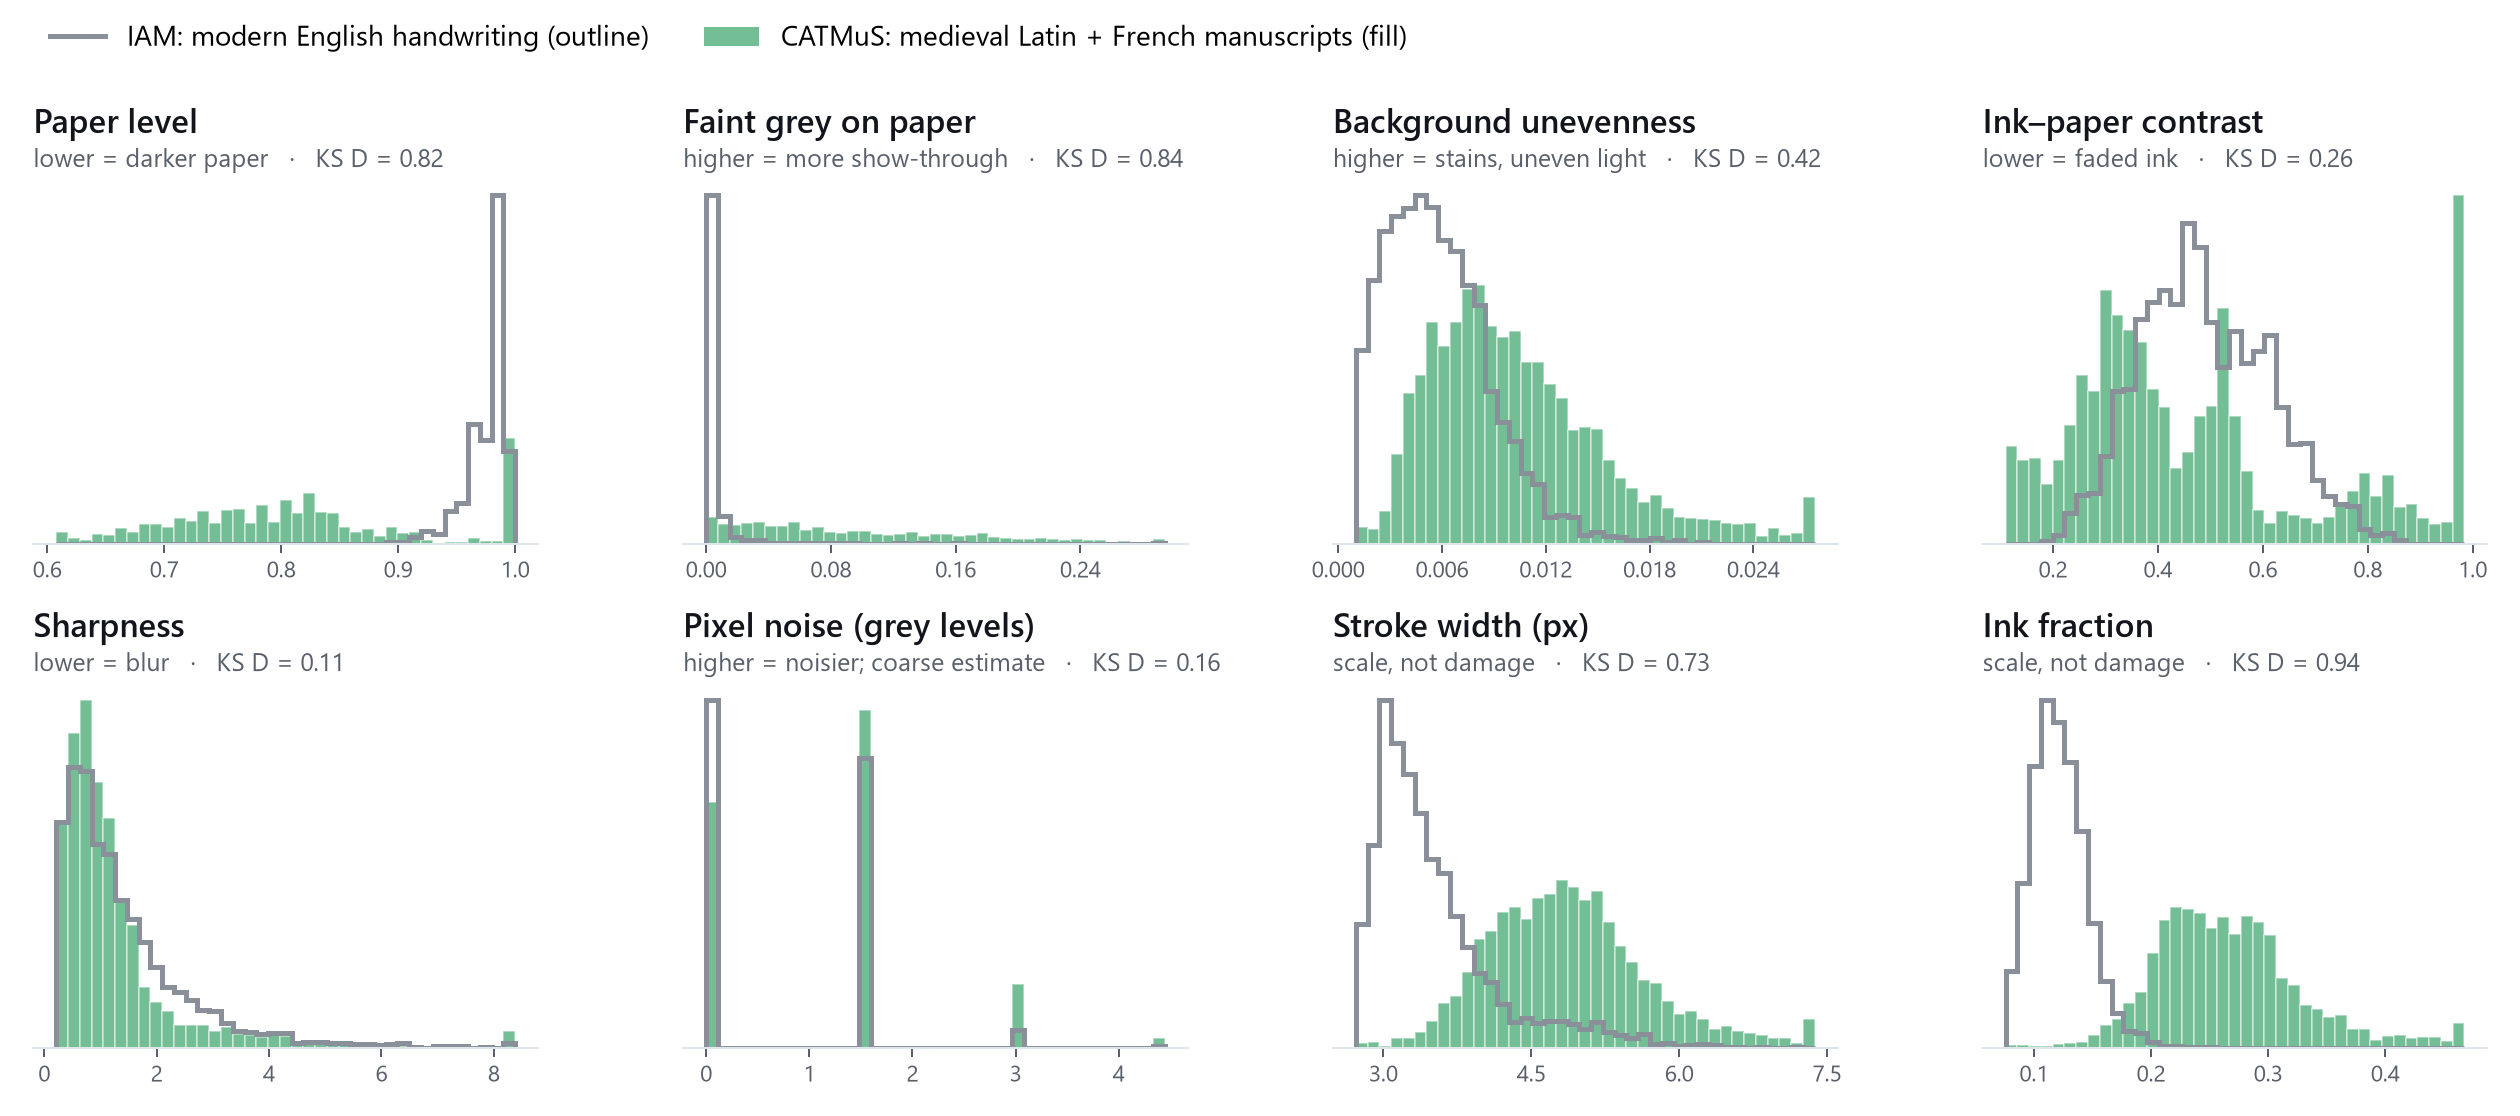
\includegraphics[width=1\linewidth,height=\textheight,keepaspectratio,alt={Distributions
of the eight line statistics on IAM (outline) and CATMuS
(filled).}]{figures/fig1_stats_iam_vs_catmus.png}
\caption{Distributions of the eight line statistics on IAM (outline) and
CATMuS (filled).}
\end{figure}

Real manuscripts differ clearly from clean lines in paper level and
show-through, and much less in the other damage statistics.

\textbf{Damage types.} Seven synthetic damage types are implemented:
paper tone, show-through, stain, fade, blur, noise and ink loss. Each
has three fixed test strengths (low, medium, high). Ink loss is held out
of every training recipe and serves as the unseen damage type.

\begin{figure}
\centering
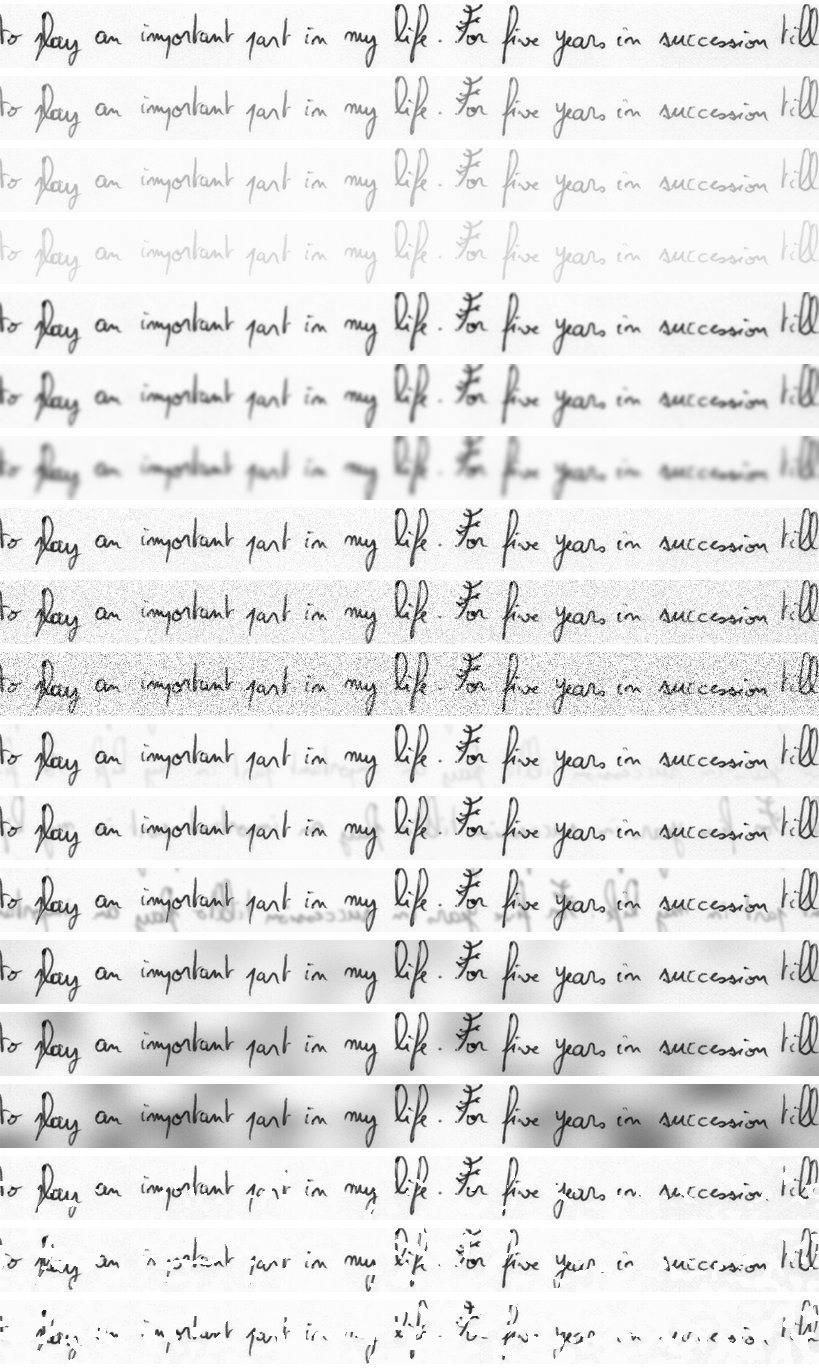
\includegraphics[width=0.5\linewidth,height=\textheight,keepaspectratio,alt={One
IAM line: clean (top), then fade, blur, noise, show-through, stain and
ink loss, each at low, medium and high
strength.}]{figures/damage_families_sheet.png}
\caption{One IAM line: clean (top), then fade, blur, noise,
show-through, stain and ink loss, each at low, medium and high
strength.}
\end{figure}

\chapter{Proposed Approach and Pilot
Results}\label{proposed-approach-and-pilot-results}

\section{Proposed Approach}\label{proposed-approach}

\begin{figure}
\centering
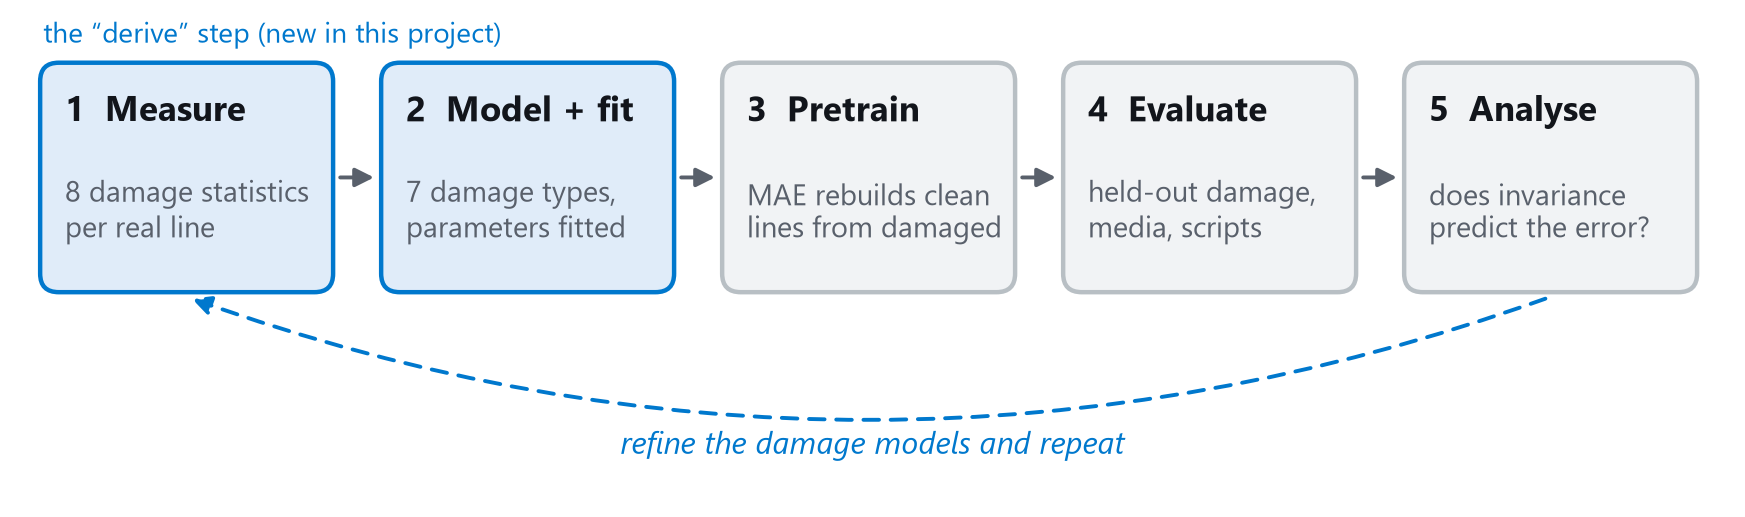
\includegraphics[width=1\linewidth,height=\textheight,keepaspectratio,alt={The
proposed pipeline. Steps 1 and 2 (measure and fit) are new in this
project.}]{figures/pipeline.png}
\caption{The proposed pipeline. Steps 1 and 2 (measure and fit) are new
in this project.}
\end{figure}

The method has five steps (Figure 6.1): measure damage statistics on
real lines; fit the frequency and strength of each damage type; pretrain
or train with the derived damage; evaluate on held-out damage, media and
scripts; and analyse whether invariance predicts the error.

\textbf{Deriving the recipe.} Each damage type is first applied to clean
IAM lines at many strengths, and its statistic is measured each time,
giving a response curve from strength to statistic. A CATMuS line counts
as damaged for a type if its statistic lies outside the 5--95\% range of
clean IAM lines. The share of such lines sets how often the damage is
applied, and their strengths, read off the response curve, set how
strong it is. The resulting recipe (v0) applies paper tone to 84\% of
lines, show-through to 89\%, stain to 37\%, fade to 26\%, noise to 11\%
and blur to 5\%. The hand-picked baseline applies each type to 50\% of
lines with a strength drawn uniformly from a range chosen by eye.

\begin{Shaded}
\begin{Highlighting}[]
\KeywordTok{def}\NormalTok{ derive(src\_stats, tgt\_stats, curves):}
\NormalTok{    out }\OperatorTok{=}\NormalTok{ \{\}}
    \ControlFlowTok{for}\NormalTok{ fam }\KeywordTok{in}\NormalTok{ FAMILIES:}
\NormalTok{        st, d }\OperatorTok{=}\NormalTok{ STAT[fam], DIRECTION[STAT[fam]]}
\NormalTok{        edge }\OperatorTok{=}\NormalTok{ src\_stats[st].quantile(}\FloatTok{0.95} \ControlFlowTok{if}\NormalTok{ d }\OperatorTok{\textgreater{}} \DecValTok{0} \ControlFlowTok{else} \FloatTok{0.05}\NormalTok{)  }\CommentTok{\# clean band}
\NormalTok{        t }\OperatorTok{=}\NormalTok{ tgt\_stats[st].dropna()}
\NormalTok{        hit }\OperatorTok{=}\NormalTok{ t[(t }\OperatorTok{\textgreater{}}\NormalTok{ edge) }\ControlFlowTok{if}\NormalTok{ d }\OperatorTok{\textgreater{}} \DecValTok{0} \ControlFlowTok{else}\NormalTok{ (t }\OperatorTok{\textless{}}\NormalTok{ edge)]  }\CommentTok{\# damaged real lines}
\NormalTok{        p }\OperatorTok{=}\NormalTok{ invert(curves[curves.family }\OperatorTok{==}\NormalTok{ fam], hit.to\_numpy())}
\NormalTok{        out[fam] }\OperatorTok{=} \BuiltInTok{dict}\NormalTok{(prob}\OperatorTok{=}\BuiltInTok{len}\NormalTok{(hit) }\OperatorTok{/} \BuiltInTok{len}\NormalTok{(t),  }\CommentTok{\# how often}
\NormalTok{                        p\_quantiles}\OperatorTok{=}\NormalTok{np.quantile(p, np.linspace(}\DecValTok{0}\NormalTok{, }\DecValTok{1}\NormalTok{, }\DecValTok{21}\NormalTok{)))}
    \ControlFlowTok{return}\NormalTok{ out                                    }\CommentTok{\# how strong}
\end{Highlighting}
\end{Shaded}

\textbf{Model.} The recogniser is a CRNN {[}1{]} with 7.4 million
parameters: a CNN that outputs 384 features per 4-pixel column, a
bidirectional LSTM and a CTC output. For pretraining, a masked
autoencoder on the CRNN's own CNN (ConvMAE) hides 60\% of the 8-pixel
vertical strips of a damaged line and learns to rebuild the clean line.
All runs share the same settings, so differences come only from the
training images.

\textbf{Invariance measure.} Each of 500 test lines is passed through
the CNN clean and with one damage added. The features are averaged along
the line, standardised using the clean lines, and compared with cosine
similarity:

\[\text{invariance} = \frac{1}{N}\sum_{i=1}^{N} \cos\big(z(x_i),\, z(\tilde{x}_i)\big) \qquad (6.1)\]

where \(x_i\) is a clean line, \(\tilde{x}_i\) the same line with damage
added, and \(z\) the standardised pooled features. A value of 1 means
the damage changed nothing inside the model.

\section{Pilot Results}\label{pilot-results}

The pilot tested four assumptions (A1 to A4), each with a pass or fail
rule written down before the runs. All results are character error rates
(CER) on the test sets; few-label results are means over two or three
random seeds.

\textbf{Baselines.} A small CRNN trained on all labels beats the
off-the-shelf commercial recogniser on both datasets (Table 6.1).

\begin{longtable}[]{@{}lll@{}}
\caption{Baseline character error rates on the test
sets.}\tabularnewline
\toprule\noalign{}
Model & IAM CER & CATMuS CER \\
\midrule\noalign{}
\endfirsthead
\toprule\noalign{}
Model & IAM CER & CATMuS CER \\
\midrule\noalign{}
\endhead
\bottomrule\noalign{}
\endlastfoot
PaddleOCR PP-OCRv6, off the shelf & 11.4\% & 52.5\% \\
CRNN, all labels & \textbf{9.8\%} & \textbf{20.0\%} \\
CRNN, few labels (IAM 10\%, CATMuS 5\%) & 19.9\% & 33.8\% \\
CRNN, very few labels (IAM 1\%) & 43.3\% & not run \\
\end{longtable}

\textbf{A1 passes: damage hurts.} On clean IAM test lines with synthetic
damage at medium strength, four of seven types more than double the
error of a clean-trained model: ink loss (9.8\% to 75.1\%), noise
(48.6\%), paper tone (33.1\%) and blur (30.2\%). On real CATMuS lines,
the quarter with the faintest ink has 1.35--1.47 times the error of the
quarter with the strongest ink.

\textbf{A2 fails: only two damage statistics differ clearly.} Paper
level (D = 0.82) and show-through (D = 0.84) pass the threshold of 0.5,
but three were required (Table 5.2). Real damage in this subset is
mainly a matter of paper tone and show-through.

\textbf{A3 fails and A4 passes: pretraining did not help.} ConvMAE
pretraining on 30,244 unlabelled lines (34 minutes) did not beat
training from scratch in any setting (CATMuS 5\%: 33.8\% scratch, 33.3\%
masking only, 35.0\% hand-picked, 33.4\% derived). Derived damage was
never worse than hand-picked damage, but only because hand-picked damage
hurt. Likely reasons, not yet tested, are the small pretraining set
(Lacuna Reconstruction used about 750,000 lines), long fine-tuning at
full learning rate, and a pretext task that is too easy.

\textbf{Derived damage as augmentation.} The same recipe was then used
without pretraining, drawing fresh damage on every labelled training
line at every pass while keeping its label.

\begin{longtable}[]{@{}
  >{\raggedright\arraybackslash}p{(\linewidth - 8\tabcolsep) * \real{0.2000}}
  >{\raggedright\arraybackslash}p{(\linewidth - 8\tabcolsep) * \real{0.2000}}
  >{\raggedright\arraybackslash}p{(\linewidth - 8\tabcolsep) * \real{0.2000}}
  >{\raggedright\arraybackslash}p{(\linewidth - 8\tabcolsep) * \real{0.2000}}
  >{\raggedright\arraybackslash}p{(\linewidth - 8\tabcolsep) * \real{0.2000}}@{}}
\caption{Damage used as training augmentation.}\tabularnewline
\toprule\noalign{}
\begin{minipage}[b]{\linewidth}\raggedright
Test CER, mean of 3 seeds
\end{minipage} & \begin{minipage}[b]{\linewidth}\raggedright
None
\end{minipage} & \begin{minipage}[b]{\linewidth}\raggedright
Hand-picked
\end{minipage} & \begin{minipage}[b]{\linewidth}\raggedright
Derived
\end{minipage} & \begin{minipage}[b]{\linewidth}\raggedright
Background filter
\end{minipage} \\
\midrule\noalign{}
\endfirsthead
\toprule\noalign{}
\begin{minipage}[b]{\linewidth}\raggedright
Test CER, mean of 3 seeds
\end{minipage} & \begin{minipage}[b]{\linewidth}\raggedright
None
\end{minipage} & \begin{minipage}[b]{\linewidth}\raggedright
Hand-picked
\end{minipage} & \begin{minipage}[b]{\linewidth}\raggedright
Derived
\end{minipage} & \begin{minipage}[b]{\linewidth}\raggedright
Background filter
\end{minipage} \\
\midrule\noalign{}
\endhead
\bottomrule\noalign{}
\endlastfoot
CATMuS 5\%, all test lines & 33.8\% & 33.6\% & \textbf{31.6\%} &
33.0\% \\
CATMuS 5\%, darkest-paper quarter & 35.6\% & 34.7\% & \textbf{33.0\%} &
35.0\% \\
CATMuS 5\%, most show-through quarter & 35.7\% & 35.1\% &
\textbf{32.9\%} & 34.7\% \\
CATMuS 5\%, lowest-contrast quarter & 39.4\% & 38.1\% & \textbf{37.0\%}
& 38.2\% \\
IAM 10\%, clean test lines & 19.9\% & \textbf{18.8\%} & 18.9\% &
19.8\% \\
\end{longtable}

On unseen medieval manuscripts, derived damage lowers the error from
33.8\% to 31.6\%, about three times the seed spread, and the gain holds
on the most damaged quarters of the test set. Hand-picked damage barely
changes the error, and a filter that flattens the paper tone reaches
only 33.0\%, so the model gains by learning to look past the damage
rather than by having it removed. On clean IAM lines the derived and
hand-picked recipes tie, as expected, since the recipe copies CATMuS
damage that clean IAM lines do not have.

\chapter{Conclusion and Plan of Work}\label{conclusion-and-plan-of-work}

\section{Conclusion of Capstone Project Phase -
1}\label{conclusion-of-capstone-project-phase---1}

Phase 1 built a reproducible pipeline for IAM and CATMuS, supervised
baselines (9.8\% CER on IAM and 20.0\% on CATMuS), a per-line damage
measurement tool, seven damage models and a first derived recipe. The
pilot checked four assumptions against rules fixed in advance. Damage
clearly hurts a clean-trained recogniser (A1 pass). Real manuscripts
differ from clean lines mainly in paper tone and show-through (A2 fail).
Reconstruction pretraining at this scale does not beat training from
scratch (A3 fail), and derived damage is never worse than hand-picked
damage (A4 pass). The strongest result is that derived damage, used as
augmentation, lowers the error on unseen medieval manuscripts from
33.8\% to 31.6\%, where hand-picked damage and a clean-up filter do not.

For the target users, archives and digital-humanities projects with few
transcribed lines, this suggests a practical procedure: measure a new
collection, derive the damage recipe from it, and train with that
recipe, instead of guessing augmentations by hand.

\section{Plan of Work for Capstone Project Phase -
2}\label{plan-of-work-for-capstone-project-phase---2}

The plan is tentative and will be confirmed with the guide.

\begin{itemize}
\tightlist
\item
  \textbf{E2, consistency training.} On unlabelled lines, the model is
  trained to give the same reading for a clean and a damaged view of a
  line. This is also the main test of H3, the sign-flip prediction.
\item
  \textbf{E3, one bounded SSL retry.} Ten times more unlabelled lines, a
  public pretrained encoder and a fixed stop date, whatever the result.
\item
  \textbf{E4, new damage.} A pair of datasets in the same script but
  with different damage, to separate the effect of damage from that of
  script.
\item
  \textbf{Damage models v1.} Physically fitted damage models, real lines
  tagged by damage type, invariance measured on CATMuS, and more seeds.
\item
  \textbf{Phase 3 stretch, script transfer.} One unseen script, such as
  an Indic script (IIIT-INDIC-HW-WORDS {[}20{]}) or Arabic manuscripts
  (Muharaf {[}21{]}), subject to access and licence.
\end{itemize}

\begin{longtable}[]{@{}
  >{\raggedright\arraybackslash}p{(\linewidth - 2\tabcolsep) * \real{0.5000}}
  >{\raggedright\arraybackslash}p{(\linewidth - 2\tabcolsep) * \real{0.5000}}@{}}
\caption{Tentative timeline for Phase 2.}\tabularnewline
\toprule\noalign{}
\begin{minipage}[b]{\linewidth}\raggedright
Period (2027)
\end{minipage} & \begin{minipage}[b]{\linewidth}\raggedright
Work
\end{minipage} \\
\midrule\noalign{}
\endfirsthead
\toprule\noalign{}
\begin{minipage}[b]{\linewidth}\raggedright
Period (2027)
\end{minipage} & \begin{minipage}[b]{\linewidth}\raggedright
Work
\end{minipage} \\
\midrule\noalign{}
\endhead
\bottomrule\noalign{}
\endlastfoot
January & Damage models v1; tag real CATMuS lines; more seeds for the
pilot runs \\
February & E2 consistency training; invariance on CATMuS (RQ3) \\
March & E3 bounded SSL retry; E4 same-script, different-damage pair
(RQ2) \\
April & Analysis, robustness checks, paper draft \\
May & Final report, demonstration and review \\
\end{longtable}

\chapter*{References}\label{references}
\addcontentsline{toc}{chapter}{References}

{[}1{]} B. Shi, X. Bai and C. Yao, ``An end-to-end trainable neural
network for image-based sequence recognition and its application to
scene text recognition,'' \emph{IEEE Transactions on Pattern Analysis
and Machine Intelligence}, vol.~39, no. 11, pp.~2298--2304, 2017.

{[}2{]} U.-V. Marti and H. Bunke, ``The IAM-database: An English
sentence database for offline handwriting recognition,''
\emph{International Journal on Document Analysis and Recognition},
vol.~5, pp.~39--46, 2002.

{[}3{]} T. Clérice \emph{et al.}, ``CATMuS Medieval: A multilingual
large-scale cross-century dataset in Latin script for handwritten text
recognition and beyond,'' in \emph{Proc. ICDAR 2024}, LNCS 14806,
Springer, 2024, pp.~174--194.

{[}4{]} C. Penarrubia, J. J. Valero-Mas and J. Calvo-Zaragoza,
``Self-supervised learning for text recognition: A critical survey,''
\emph{International Journal of Computer Vision}, 2025.

{[}5{]} M. Kišš and M. Hradiš, ``Self-supervised pre-training of text
recognizers,'' in \emph{Proc. International Conference on Document
Analysis and Recognition (ICDAR)}, 2024.

{[}6{]} N. Vogler, J. P. Allen, M. T. Miller and T. Berg-Kirkpatrick,
``Lacuna reconstruction: Self-supervised pre-training for low-resource
historical document transcription,'' in \emph{Findings of the
Association for Computational Linguistics: NAACL 2022}, 2022.

{[}7{]} K. He, X. Chen, S. Xie, Y. Li, P. Dollár and R. Girshick,
``Masked autoencoders are scalable vision learners,'' in \emph{Proc.
IEEE/CVF CVPR}, 2022, pp.~16000--16009.

{[}8{]} C. Garrido-Munoz and J. Calvo-Zaragoza, ``Handwritten text
recognition lives in the high-pixel variance subspace,''
arXiv:2609.35473, 2026.

{[}9{]} PaddlePaddle Authors, ``PaddleOCR (PP-OCR series),'' GitHub
repository. {[}Online{]}. Available:
https://github.com/PaddlePaddle/PaddleOCR

{[}10{]} A. Aberdam, R. Litman, S. Tsiper, O. Anschel, R. Slossberg, S.
Mazor, R. Manmatha and P. Perona, ``Sequence-to-sequence contrastive
learning for text recognition,'' in \emph{Proc. IEEE/CVF CVPR}, 2021.

{[}11{]} Mitra, Mondal and C. V. Jawahar, ``Learning beyond labels:
Self-supervised handwritten text recognition,'' in \emph{Proc. IEEE/CVF
WACV}, 2026, pp.~6653--6663.

{[}12{]} M. A. Souibgui, S. Biswas, A. Mafla, A. F. Biten, A. Fornés, Y.
Kessentini, J. Lladós, L. Gomez and D. Karatzas, ``Text-DIAE: A
self-supervised degradation invariant autoencoder for text recognition
and document enhancement,'' in \emph{Proc. AAAI Conference on Artificial
Intelligence}, 2023.

{[}13{]} T. Kanungo, R. M. Haralick, H. S. Baird, W. Stuetzle and D.
Madigan, ``A statistical, nonparametric methodology for document
degradation model validation,'' \emph{IEEE Transactions on Pattern
Analysis and Machine Intelligence}, vol.~22, no. 11, pp.~1209--1223,
2000.

{[}14{]} H. S. Baird, ``The state of the art of document image
degradation modelling,'' in \emph{Digital Document Processing}, B. B.
Chaudhuri, Ed. London: Springer, 2007, pp.~261--279.

{[}15{]} A. Groleau, K. W. Chee, S. Larson, S. Maini and J. Boarman,
``Augraphy: A data augmentation library for document images,'' in
\emph{Proc. ICDAR 2023}; arXiv:2208.14558.

{[}16{]} Guan, Lin, Xu, Liu, Zhao, Fan, Xu and Greene, ``PreP-OCR: A
complete pipeline for document image restoration and enhanced OCR
accuracy,'' in \emph{Proc. Annual Meeting of the Association for
Computational Linguistics (ACL)}, 2025.

{[}17{]} L. Ericsson, H. Gouk and T. M. Hospedales, ``Why do
self-supervised models transfer? On the impact of invariance on
downstream tasks,'' in \emph{Proc. British Machine Vision Conference
(BMVC)}, 2022.

{[}18{]} E. Mintun, A. Kirillov and S. Xie, ``On interaction between
augmentations and corruptions in natural corruption robustness,'' in
\emph{Advances in Neural Information Processing Systems (NeurIPS)},
2021.

{[}19{]} A. Bardes, J. Ponce and Y. LeCun, ``VICReg:
Variance-invariance-covariance regularization for self-supervised
learning,'' in \emph{Proc. International Conference on Learning
Representations (ICLR)}, 2022.

{[}20{]} S. Gongidi and C. V. Jawahar, ``IIIT-INDIC-HW-WORDS: A dataset
for Indic handwritten text recognition,'' in \emph{Proc. ICDAR 2021},
2021.

{[}21{]} M. Saeed \emph{et al.}, ``Muharaf: Manuscripts of handwritten
Arabic dataset for cursive text recognition,'' in \emph{NeurIPS 2024
Datasets and Benchmarks Track}, 2024.

\chapter*{Appendix A: Definitions, Acronyms and
Abbreviations}\label{appendix-a-definitions-acronyms-and-abbreviations}
\addcontentsline{toc}{chapter}{Appendix A: Definitions, Acronyms and
Abbreviations}

{\def\LTcaptype{none} % do not increment counter
\begin{longtable}[]{@{}
  >{\raggedright\arraybackslash}p{(\linewidth - 2\tabcolsep) * \real{0.5000}}
  >{\raggedright\arraybackslash}p{(\linewidth - 2\tabcolsep) * \real{0.5000}}@{}}
\toprule\noalign{}
\begin{minipage}[b]{\linewidth}\raggedright
Term
\end{minipage} & \begin{minipage}[b]{\linewidth}\raggedright
Meaning
\end{minipage} \\
\midrule\noalign{}
\endhead
\bottomrule\noalign{}
\endlastfoot
Augmentation & Changing a training image (here, adding synthetic damage)
while keeping its label \\
CER & Character error rate: edit distance between prediction and true
text, divided by the length of the true text \\
ConvMAE & Masked autoencoder built on the CRNN's own CNN, used for
pretraining in this project \\
CRNN & Convolutional recurrent neural network: CNN, then BiLSTM, then
CTC \\
CTC & Connectionist temporal classification; a loss that aligns a
sequence of predictions with the target text \\
Derived recipe & Frequency and strength of each damage type, set from
measurements of real lines \\
HTR & Handwritten text recognition \\
Invariance & How little a model's internal features change when a damage
is added (1 = no change) \\
KS distance (D) & Kolmogorov--Smirnov statistic: largest gap between two
cumulative distributions (0 = same, 1 = separate) \\
MAE & Masked autoencoder: hides parts of an image and learns to rebuild
them \\
Seed & The starting value of the random number generator; repeating a
run with different seeds shows how much results vary by chance \\
Show-through & Ink from the reverse side of the page visible through the
paper \\
SSL & Self-supervised learning: learning from data without labels
through a pretext task \\
\end{longtable}
}

\end{document}
